\section{Compiler}\label{sec:compiler}

Damit eine Programmiersprache verwendbar ist, muss sie nicht nur eine Spezifikation haben, sondern auch ausführbar sein.
Dies kann durch direktes Ausführen des Programmtexts geschehen;
in diesem Fall wird das ausführende Programm Interpreter genannt.
Andererseits kann eine Programmiersprache auch in ein maschinenlesbares Format übersetzt werden,
das dann direkt oder durch eine virtuelle Maschine ausgeführt wird.
Dieser Ansatz nennt sich Kompilierung.
In Java wird die Kompilierung durch den Java Compiler (\code{javac}) durchgeführt, welcher Bytecode erzeugt;
dieser kann von einer Java Virtual Machine (JVM) ausgeführt werden.

FulibScenarios wird hingegen in zwei Schritten kompiliert.
Zunächst werden die Markdown-Scenario-Quelltexte in Java-Quelltexte übersetzt;
dies ist Aufgabe des Scenario-Compilers.
Der erzeugte Java-Quellcode wird dann vom Java-Compiler kompiliert.
Die Architektur und Implementierung des Scenario-Compilers sind Inhalt dieses Abschnitts.
Dabei wird des öfteren auf das Beispiel in Listing~\ref{lst:CompilationExample.md} Bezug genommen,
dessen Übersetzung bis zum Java-Quellcode in den einzelnen Teilabschnitten stückweise erarbeitet wird.

\codelisting{md}{chapter/fulib-scenarios/scenarios}{CompilationExample.md}{Beispiel-Szenario für diesen Abschnitt, gespeichert als \code{src/main/scenarios/org/example/CompilationExample.md}}

\subsection{Architektur}\label{subsec:compiler-architecture}

\todo{
    Visitor Pattern~\cite{gof-design-patterns}.
    Dragon Book~\cite{dragonbook}.
}

\begin{figure}
    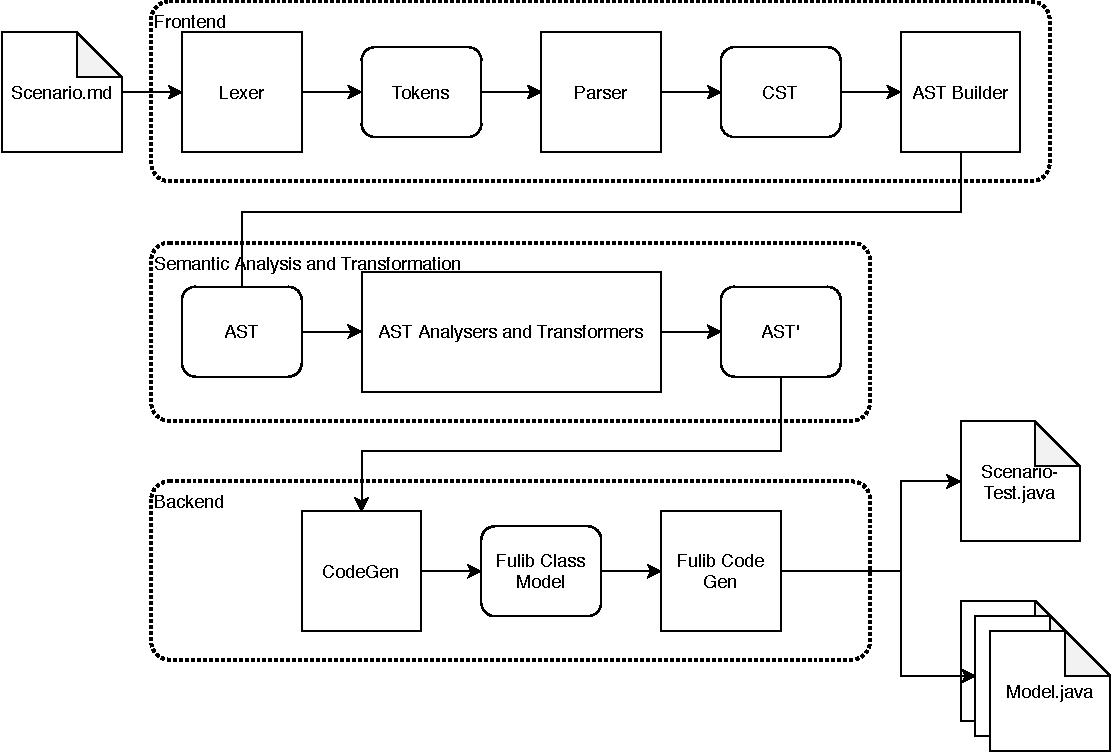
\includegraphics[width=\textwidth]{chapter/fulib-scenarios/img/architecture.pdf}
    \caption{Compiler-Architektur}
    \label{fig:compiler-architecture}
\end{figure}

\subsection{Frontend - ANTLR v4}\label{subsec:frontend-antlr4}

Die Übersetzung der Markdown-Datei beginnt mit deren Einlesen und Umwandeln in verarbeitbare Daten.
Im Compilerbau wird dies klassisch in zwei Phasen unterteilt:
Dem \emph{Lexer}, der die Zeichenfolge in eine Liste von Wörtern mit Typinformationen, genannt \emph{Tokens}, umwandelt;
und dem \emph{Parser}, der die flache Liste von Tokens nach den Regeln der Grammatik in eine Baumstruktur bringt,
die \emph{Concrete Syntax Tree (CST)} genannt wird.

Da die Umwandlung in Tokens und deren Strukturierung Anwendung in den meisten Compilern findet
und deren Implementierung meist nach einem festen Muster stattfindet,
existieren Tools, die diesen Prozess vereinfachen.
Diese werden \emph{Compiler-Compiler} oder \emph{Lexer- und Parsergeneratoren} genannt.

Das Frontend des Scenario-Compilers basiert auf dem Parsergenerator ANTLR4~\cite{antlr4-reference}.
Mit diesem können Grammatiken in einem EBNF-ähnlichen Format spezifiziert werden.
Aus der Grammatik generiert das Tool dann Java-Code, der Dateien einlesen kann und einen CST generiert.

Zunächst soll betrachtet werden, wie die FulibScenarios-Grammatik definiert ist.
Dies beginnt mit der Definition des Lexers.
In Listing~\ref{lst:ScenarioLexer.g4} ist ein Ausschnitt der ANTLR4-Grammatik zu sehen, die diesen definiert.
Der Ausschnitt ist ausreichend um das Scenario aus Listing~\ref{lst:CompilationExample.md} verarbeiten zu können;
die eigentliche Grammatik von FulibScenarios besteht aus vielen weiteren Regeln, um alle Funktionen der Sprache zu implementieren.
Sie ist in Anhang~\ref{sec:scenario-lexer-grammar} zu finden.

\codelisting{antlr}{chapter/fulib-scenarios/grammars}{ScenarioLexer.g4}{Ausschnitt der Scenario-Lexer-Grammatik}

Die Grammatik besteht aus mehreren Regeln, die einem Muster einen Namen zuordnen.
Dieser Name wird später den Tokens zugeordnet.
So haben Tokens mit dem Text \code{and} später den Namen \code{AND};
und jene, die eine Zahl darstellen, den Namen \code{INTEGER}.
Im Folgenden werden Tokens mit der Kurzschreibweise \code{<name>(<text>)} bezeichnet,
z.B.\ \code{AND(and)} und \code{INTEGER(12)}.

Die rechte Seite jeder Regel ähnelt einem regulären Ausdruck.
Bei Schlüsselwörtern wie \code{a}, \code{is} und \code{with} muss der Text exakt entsprechen;
\code{There} darf beispielsweise auch kleingeschrieben werden.
Ein \code{HEADLINE}-Token entsteht, wenn auf ein \code{#}-Zeichen beliebig viele Zeichen und ein Zeilenumbruch folgen.
Ganze Zahlen können mit einem Minus-Zeichen beginnen und bestehen aus mindestens einer Ziffer.
Wörter beginnen mit einem Buchstaben, gefolgt von beliebig vielen Buchstaben, Ziffern, Apostrophen, Unterstrichen und Bindestrichen.
Die Regel \code{WS} sorgt durch die Angabe \code{-> skip} dafür, dass keine Whitespace-Zeichen zu Token werden.
Falls mehrere Regeln infrage kommen würden, wird zunächst die längstmögliche Übereinstimmung angewandt;
falls das nicht eindeutig bestimmbar ist, gewinnt die als erste definierte Regel.
So wird aus dem Text \code{ampersand} nicht die Token-Folge \code{A(a), WORD(mpers), AND(and)}, sondern \code{WORD(ampersand)}.

Wendet man die Regeln aus Listing~\ref{lst:ScenarioLexer.g4} auf das Scenario aus Listing~\ref{lst:CompilationExample.md} an,
so erhält man die in Listing~\ref{lst:CompilationExampleTokens.txt} gezeigte Liste von Tokens.

\codelisting{text}{chapter/fulib-scenarios/trees}{CompilationExampleTokens.txt}{Aus Listing~\ref{lst:CompilationExample.md} abgeleitete Token-Liste}

Als nächstes sollen diese Tokens in einen CST umgewandelt werden.
Dies ist die Aufgabe des Parsers.
Listing~\ref{lst:ScenarioParser.g4} zeigt wieder einen Ausschnitt der Grammatik,
die diesen für das Beispiel-Scenario ausreichend definiert.
Die vollständige Parser-Grammatik ist Inhalt von Anhang~\ref{sec:scenario-parser-grammar}.

\codelisting{antlr}{chapter/fulib-scenarios/grammars}{ScenarioParser.g4}{Ausschnitt der Scenario-Parser-Grammatik}

Die Struktur der Parser-Grammatik ist ähnlich zur Lexer-Grammatik.
Wieder gibt es benannte Regeln, jedoch bestehen deren rechte Seite nicht aus regulären Ausdrücken,
sondern aus \emph{Nicht-Terminal}-Symbolen, die weitere Parser-Regeln referenzieren\footnote{Diese sind in der ANTLR-Grammatik daran zu erkennen, dass sie mit einem Kleinbuchstaben beginnen.},
sowie \emph{Terminal}-Symbolen, die analog Verweise auf Lexer-Regeln sind\footnote{In ANTLR beginnen diese immer mit einem Großbuchstaben.}.
Die \code{thereSentence}-Regel aus Listing~\ref{lst:ScenarioParser.g4} beginnt beispielsweise mit den Terminalen \code{THERE}, \code{IS}, \code{A} und \code{WORD}, gefolgt von dem Nicht-Terminal \code{withClause}.
Beim Ableiten eines konkreten Syntaxbaumes werden alle Terminale zu den Blättern;
die Nicht-Terminale werden zu Elternknoten.

In Listing~\ref{lst:ScenarioParser.g4} dient \code{file} als Startregel.
Nun wird diese Regel \emph{abgeleitet}, d.h.\ die Tokens, die derzeit am Anfang unserer Liste stehen, werden entweder einem Terminal zugeordnet oder ein Nicht-Terminal wird rekursiv abgeleitet.
Da \code{file} mit dem Nicht-Terminal \code{heading} beginnt, wird zunächst dieses abgeleitet.
Dabei wird dem Terminal \code{HEADLINE} das Token \code{HEADLINE(# My First Scenario)} zugeordnet.
Als nächstes werden \code{sentence} und \code{thereSentence} abgeleitet, wobei den Terminalen \code{THERE}, \code{IS} und \code{A} und \code{WORD} das entsprechende Token zugeordnet wird.
Bei der Ableitung von \code{withClause} muss entschieden werden, welche Alternative der Regel zutrifft.
Im Fall von dem Teilsatz \code{with name Alice} wird die erste Alternative ausgewählt, da \code{name} ein \code{WORD}-Token ist und nicht dem \code{INTEGER}-Terminal zugeordnet werden kann.
Der Ausdruck \code{withClause (AND withClause)*} in der \code{thereSentence}-Regel bedeutet, dass auf eine \code{with}-Klausel beliebig viele weitere \code{with}-Klauseln folgen können, solange dazwischen ein \code{AND}-Token steht.
Da dies im Beispiel der Fall ist, wird \code{AND(and)} dem \code{AND}-Terminal zugeordnet und \code{withClause} erneut abgeleitet.
Diesmal wird dabei die zweite Alternative gewählt, da \code{INTEGER(30)} dem \code{INTEGER}-Terminal zugeordnet werden kann.
Zuletzt wird der Punkt am Ende des Satzes dem \code{FULL_STOP}-Terminal zugeordnet.

Nun sind alle Token, die der Lexer aus der Eingabe produziert hat, verbraucht, und der Parse-Vorgang ist abgeschlossen.
Das Ergebnis ist der in Abbildung~\ref{fig:parsetree} sichtbare Syntaxbaum.

\begin{figure}
    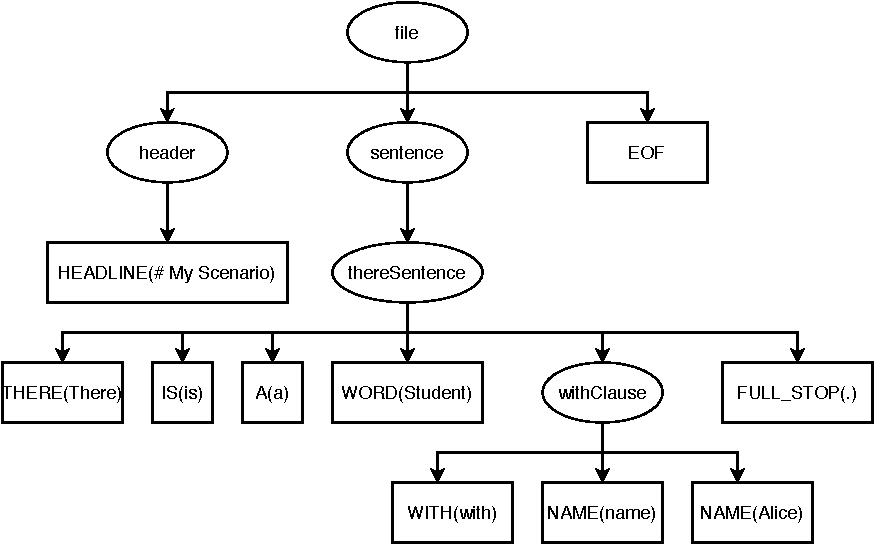
\includegraphics[width=\textwidth]{chapter/fulib-scenarios/img/parsetree.pdf}
    \caption{Syntaxbaum von Listing~\ref{lst:CompilationExample.md}}
    \label{fig:parsetree}
\end{figure}

Der CST ist eng an die Struktur der Grammatik gebunden.
Bei Änderungen an der Grammatik, beispielsweise dem Einfügen von gemeinsamen Hilfsregeln beim Refactoring,
ändert sich auch die Struktur des CST\@.
Würde man also den CST für weitere Schritte des Compile-Vorgangs verwenden,
müsste man die Implementierung dieser Schritte bei Änderung der Grammatik an die neue CST-Struktur anpassen,
was zu einem Wartungsproblem führt.

Deshalb hat das Frontend zusätzlich die Aufgabe, den CST in eine umgänglichere Form umzuwandeln.
Diese nennt man \emph{Abstract Syntax Tree} (AST).
Die Namensgebung folgt daher, dass über die Grammatik abstrahiert wird.

Technisch gesehen besteht der AST aus einem weiteren Datenmodell neben dem Datenmodell des Parsers.
Während letzteres von ANTLR aus der Grammatik hergeleitet und generiert wird,
ist das Datenmodell des AST manuell definiert und am logischen Aufbau eines Szenarios orientiert.
So gibt es AST-Klassen für Pakete, Dateien, Scenarios in Dateien und jegliche Arten von Sätzen und Ausdrücken.
Für bestimmte Konstrukte, die in mehreren Sätzen vorkommen, gibt es Hilfsklassen um Code-Duplizierung zu vermeiden.
Dazu gehören z.B.\ mit Namen versehene Ausdrücke.

Das Datenmodell des AST wird ebenfalls automatisch generiert.
Grund dafür ist, dass jede AST-Klasse lediglich aus Klassenvariablen, Gettern und Settern sowie einer Factory-Methode besteht.
Diese können mit einer Liste von Attributen ausreichend definiert werden.

Die Generierung des AST erfolgt durch das GenTreeSrc-Tool~\cite{gentreesrc}.
Dieses erlaubt die Definition von Klassen und Attributen in einer \code{gts}-Datei,
aus der dann Java-Dateien generiert werden.
Listing~\ref{lst:FulibScenarios.gts} zeigt einen Ausschnitt der \code{gts}-Datei von FulibScenarios,
in dem die für Beispiel~\ref{lst:CompilationExample.md} benötigten Definitionen abgebildet sind.
Die vollständige Definitionsdatei ist in Anhang~\ref{sec:gts-definitions} zu finden.

\codelisting{java}{chapter/fulib-scenarios/definitions}{FulibScenarios.gts}{Ausschnitt der FulibScenarios.gts-Datei}

Diese Datei verwendet die Syntax von GenTreeSrc, welche wie folgt zu lesen ist:
Auf der obersten Ebene werden Klassen inkl.\ Package-Name definiert, z.B. \code{org.fulib.scenarios.ast.Node}.
Das Schlüsselwort \code{abstract} bedeutet hier, dass diese ein Interface ist und nicht instanziiert werden kann.
In den geschweiften Klammern nach einer Klassendefinition werden weitere Klasse definiert, die von dieser erben.
Diese werden entweder im selben Package (\code{org.fulib.scenarios.ast.ScenarioFile}) oder in einem Unterpackage
(\code{org.fulib.scenarios.ast.decl.Name}) abgelegt.
Runde Klammern nach dem Klassennamen enthalten die Attribute, die die Syntax \code{name: Typ} verwenden.
Die Typausdrücke \code{[T]} und \code{[T:U]} stehen für \code{List<T>} und \code{Map<T, U>}.
Einfache Attribute haben einen Getter und Setter;
das Schlüsselwort \code{readonly} sorgt dafür, dass kein Setter erzeugt wird.
Aus jedem Attribut wird ein Parameter im Konstruktor bzw.\ der Factory-Methode der generierten Klasse.

Mit den generierten Klassen kann nun ein AST erzeugt werden.
Dafür implementiert das Frontend einen Übersetzungsschritt für eine Vielzahl von CST-Knoten,
der diese bei den Blättern beginnend in AST-Knoten umwandelt.

Ergebnis der Übersetzung des in Abbildung~\ref{fig:parsetree} gezeigten CST ist der AST,
der in Listing~\ref{lst:CompilationExampleAST.txt} in seinem Ausgabeformat dargestellt ist\footnote{
    Im Scenario-Compiler steht auf der obersten Ebene ein \code{CompilationContext}-Knoten, der u.a.\ Kompilierungsoptionen enthält.
    Darunter befinden sich Knoten für Pakete;
    erst diese enthalten den \code{ScenarioFile}-Knoten.
    Aus Gründen der Einfachheit wurden diese beiden Ebenen hier ausgelassen.
}.

\codelisting{java}{chapter/fulib-scenarios/trees}{CompilationExampleAST.txt}{AST von Listing~\ref{lst:CompilationExample.md}}

\subsection{Analyse und Transformation}\label{subsec:data-model-gentreesrc}

Sobald der AST im Frontend erzeugt wurde, beginnt die Analyse- und Transformationsphase.
Deren Aufgabe ist es, den AST auf semantische Gültigkeit zu überprüfen und ihn so vorzubereiten,
dass in der folgenden Codegenerierungsphase alle Informationen bereitstehen.

Bei der Analyse werden die Fehler- und Warnmeldungen erzeugt, die die Ausgabe des Compilers bilden.
Dafür werden im AST durch das Frontend Positionsinformationen von Tokens hinterlegt, die es ermöglichen,
in den Meldungen Dateinamen, Zeilen- und Spaltennummern einzubringen.
Die entsprechenden Attribute in AST-Klassen wurden hier zur Einfachheit ausgelassen,
sie sind jedoch in Anhang~\ref{sec:gts-definitions} enthalten.

Die Analyse- und Transformationphase besteht im Scenario-Compiler aus zwei logisch getrennten Unterphasen,
der Gruppierung und der Namensauflösung.
Die Gruppierung ist zuständig dafür, aus der linearen Abfolge von Sätzen in einem Scenario eine Baumstruktur zur erzeugen,
wenn Sätze anderen untergeordnet werden können.
Dies ist beispielsweise bei jenen der Fall, die unter einem \todo{Call/Tell}-Satz stehen, welche im vorherigen Abschnitt unter~\ref{subsec:methods} näher erläutert wurden.
Jeder Satz, dessen Akteur dem \todo{Call/Tell}-Satz entspricht, wird diesem untergeordnet und ist nicht länger direkt Teil der Satzliste des Scenarios.
Grund dafür ist, dass der Code für diese Sätze später nicht im Test, sondern in der entsprechenden Methode auftaucht.
Da für die Bestimmung von Akteuren keine komplexe Namensauflösung notwendig ist,
die Unterordnung von Sätzen jedoch deren Scope beeinflusst, geschieht die Gruppierung vor der Namensauflösung.

Die Namensauflösung bündelt sowohl die direkte Namensauflösung anhand des Scopes,
als auch die Auflösung von Attributen und Assoziationen, das Erzeugen von Klassen, das Erzeugen von Diagnosenachrichten,
und die Umstrukturierung des AST\@.
Grund dafür ist, dass diese Aufgaben eng verzahnt und meist in einem Schritt ausführbar sind.
Beim Auflösen von Assoziation beispielsweise kann diese angelegt werden, falls es sie noch nicht gibt,
andernfalls kann die bestehene Assoziation auf Konflikte überprüft werden und ggf.\ eine Fehlermeldung erzeugt werden.
\todom{Beispiel?}

Des Weiteren ist es meist vorteilhaft, den AST vor der Auflösung zu vereinfachen.
Bildet man beispielsweise eine Art von AST-Knoten immer auf eine andere ab,
müssen folgende Schritte nicht mehr für die erste Knotenart implementiert werden,
da man sichergehen kann, dass sie nicht mehr vorkommt.
Dadurch kann Code-Duplizierung vermieden und die Code-Generierung vereinfacht werden.
\todom{"Siehe Beispiel im nächsten Abschnitt"?}

Es soll nun der im vorherigen Abschnitt angelegte AST, der in Listing~\ref{lst:CompilationExampleAST.txt} gezeigt wurde, weiter verarbeitet werden.
Da die Gruppierung in diesem Beispiel keine Veränderungen durchführt, können wir als nächstes die Namensauflösung betrachten.
Dabei führt der Scenario-Compiler zunächst einen Umformungsschritt durch, der den \code{ThereSentence} durch einen \code{IsSentence} und einen \code{HasSentence} ersetzt.
Diese Umformung erhält die Semantik, dass ein Objekt angelegt und einer Variable zugewiesen wird und daraufhin ein Attribut gesetzt wird,
wie im vorherigen Abschnitt unter~\ref{subsec:simple-sentences-and-expressions} gezeigt wurde.
In Listing~\ref{lst:PreprocessedAST.txt} ist der AST nach dieser Umformung abgebildet.
Zur Vereinfachung ist nur der \code{Scenario}-Knoten gezeigt;
der \code{ScenarioFile}- sowie darüberliegende Knoten bleiben unverändert.
Listing~\ref{lst:FulibScenarios2.gts} zeigt die neuen AST-Klassendefinitionen, die dafür notwendig sind.

\codelisting{java}{chapter/fulib-scenarios/trees}{PreprocessedAST.txt}{AST nach Umformung von \code{ThereSentence} zu \code{IsSentence} + \code{HasSentence}}

\codelisting{java}{chapter/fulib-scenarios/definitions}{FulibScenarios2.gts}{Neue AST-Klassendefinitionen für Listing~\ref{lst:PreprocessedAST.txt}}

Im nächsten Schritt werden die neu erzeugten \code{Sentence}-Knoten aufgelöst.
Meist ist an dem Wort \code{Unresolved} zu erkennen, dass ein AST-Knoten aufgelöst werden muss.
Im \code{IsSentence}-Knoten fällt dabei der \code{type} der \code{CreationExpr} auf.

Der Compiler verwendet für die Auflösung einen Scope, der aus mehreren Ebenen besteht die jeweils Deklarationen bereitstellen können.
Beim Auflösen eines Namens wird beginnend beim inneren Scope eine Deklaration mit diesem Namen gesucht;
falls dies kein Ergebnis liefert wird im jeweils nächstäußeren Scope gesucht.
Gelangt man im äußersten Scope an ohne eine Deklaration gefunden zu haben,
kann diese automatisch erzeugt werden oder eine Fehlermeldung generiert werden.
Dies findet wieder auf der zuständigen Scope-Ebene statt.

Die Scope-Hierarchie ist im Fall der \code{CreationExpr} von außen nach innen wie folgt:
Global, Paket, Scenario-Datei, Scenario, Satz-Liste.
Dabei ist die Satz-Liste für das Auflösen und Anlegen von lokalen Variablen zuständig,
die Scenario-Datei und Paket enthalten Hilfsmethoden bzw.\ Klassen,
und der globale Scope stellt extern importierte Klassen bereit.
Wird nun versucht, den Typnamen \code{Student} in diesem Scope aufzulösen,
findet man zunächst keine entsprechende Deklaration.
Deshalb wird ein neues Objekt im Datenmodell des Compilers angelegt,
das die Klasse \code{Student} repräsentiert und deren Zugehörigkeit zum gleichen Paket wie die Scenario-Datei darstellt.
Der \code{UnresolvedType}-Knoten wird zu einem \code{ClassType}, der auf diese neue Klasse verweist.
Nun ist der Typ der \code{CreationExpr} aufgelöst und kann als Typ der Variable \code{alice} inferiert werden.

Als nächstes müssen die beiden \code{UnresolvedName}s im \code{HasSentence} einer Deklaration zugeordnet werden.
\todom{"Alice" wird Objekt ID und Var.}
Der \code{HasSentence} fügt der Scope-Hierarchie eine weitere Ebene hinzu, die den Namen \code{alice} \emph{versteckt}.
Deshalb wird die gleichnamige Variable \emph{nicht} dem \code{UnresolvedName} zugeordnet.
Wäre dies der Fall, würde der \code{has}-Satz eine Assoziation von \code{Student} zu sich selbst erzeugen,
was offensichtlich nicht gewollt ist.
Da \code{alice} nicht aufgelöst werden kann, wird aus dem \code{NameAccess} hier ein \code{StringLiteral}.

Die Auflösung von \code{UnresolvedName(value: "name")} als Teil der \code{NamedExpr} wird besonders gehandhabt.
\todom{"name" wird Attribut von Student}
Hier erfolgt nicht wie üblich eine Suche im aktuellen Scope,
sondern im Typ des Empfängers, also des \code{object}s des \code{HasSentence}.
Dies ist der Typ der Variable \code{var1}, der beim Auflösen des \code{IsSentence} als der Klassentyp \code{Student} inferiert wurde.
Nun wird in diesem nach einem Attribute oder einer Assoziation namens \code{name} gesucht.
Wäre eines davon bereits vorhanden, würde der Compiler diverse Überprüfungen durchführen,
ob diese mit dem Typ des Attributwerts kompatibel sind.
Da die Klasse \code{Student} jedoch \todom{in unserem Beispiel} noch keine Attribute oder Assoziationen hat,
wird ein neues Attribute mit dem Namen \code{name} und dem Typ \code{String} angelegt
und im Datenmodell der Klasse \code{Student} gespeichert.
Daraufhin wird der \code{UnresolvedName} durch einen \code{ResolvedName} ausgetauscht,
der auf das neue Attribute verweist.

Die Analyse und Transformation des AST ist nun abgeschlossen.
Listing~\ref{lst:FinalAST.txt} zeigt den vollständigen AST, der nun für die Codegenerierung vorbereitet ist.
Die darin verwendeten neuen AST-Definitionen sind in Listing~\ref{lst:FulibScenarios3.gts} zu finden.

\codelisting{java}{chapter/fulib-scenarios/trees}{FinalAST.txt}{AST nach Analyse und Transformation}

\codelisting{java}{chapter/fulib-scenarios/definitions}{FulibScenarios3.gts}{Für Auflösung und vollständingen AST benötigte AST-Definitionen}

\subsection{Codegenerierung - Fulib}\label{subsec:codegen-fulib}

Die letzte Aufgabe des Scenario-Compilers ist die Codegenerierung.
Dabei werden mit den in vorherigen Phasen gesammelten Informationen neue Java-Dateien erzeugt bzw.\ bestehende verändert.
Der Scenario-Compiler verwendet für diesen Zweck die Fulib\cite{fulib}-Bibliothek.
Diese stellt wie der Scenario-Compiler ein Datenmodell für Klassen, Attributen, Assoziationen und Methoden bereit,
bietet aber auch deren Umwandlung in Java-Code an.
Der Codegenerator von Fulib unterstützt dabei das Zusammenführen von bestehenden Java-Dateien mit neu generiertem Code,
wodurch er mit handgeschriebenem Code kompatibel ist.

Die Aufgabe des Codegenerators des Scenario-Compilers ist es also \emph{nicht},
Java-Dateien anzulegen und zeilenweise auszufüllen;
dies wird an Fulib delegiert.
Dazu konvertiert der Scenario-Compiler sein internes, an die Scenario-Sprache angepasstes Datenmodell in das Datenmodell von Fulib.
Für Klassen, Attribute und Assoziationen ist diese Umwandlung annähernd 1-zu-1;
lediglich Methoden werden gesondert gehandhabt.
Grund dafür ist, dass das Datenmodell von Fulib zwar Methodendeklarationen versteht,
deren Rumpf jedoch als Zeichenkette modelliert,
da es kein Modell für Anweisungen und Ausdrücke bereitstellt.
Der Scenario-Compiler ist also dafür zuständig, Methodenrümpfe zeilenweise zusammenzusetzen.

Ferner sieht der Scenario-Codegenerator eine logische Trennung von Modell und Tests vor.
Fulib selbst kennt diese Trennung nicht, daher erzeugt der Scenario-Compiler zwei getrennte Fulib-Datenmodelle, welche später auch in getrennte Verzeichnisse Java-Dateien ablegen.

\todo{
    Modellgenerierung mit Fulib.
    Testgenerierung selbst.
}
